
%%%
% Plantilla de Memoria
% Modificación de una plantilla de Latex de Nicolas Diaz para adaptarla 
% al castellano y a las necesidades de escribir informática y matemáticas.
%
% Editada por: Mario Román
%
% License:
% CC BY-NC-SA 3.0 (http://creativecommons.org/licenses/by-nc-sa/3.0/)
%%%

%%%%%%%%%%%%%%%%%%%%%%%%%%%%%%%%%%%%%%%%%
% Thin Sectioned Essay
% LaTeX Template
% Version 1.0 (3/8/13)
%
% This template has been downloaded from:
% http://www.LaTeXTemplates.com
%
% Original Author:
% Nicolas Diaz (nsdiaz@uc.cl) with extensive modifications by:
% Vel (vel@latextemplates.com)
%
% License:
% CC BY-NC-SA 3.0 (http://creativecommons.org/licenses/by-nc-sa/3.0/)
%
%%%%%%%%%%%%%%%%%%%%%%%%%%%%%%%%%%%%%%%%%

%----------------------------------------------------------------------------------------
%	PAQUETES Y CONFIGURACIÓN DEL DOCUMENTO
%----------------------------------------------------------------------------------------
%%% Configuración del papel.
% microtype: Tipografía.
% mathpazo: Usa la fuente Palatino.
\documentclass[a4paper, 11pt]{article}
\usepackage[protrusion=true,expansion=true]{microtype}
\usepackage{mathpazo}


% Indentación de párrafos para Palatino
\setlength{\parindent}{0pt}
  \parskip=8pt
\linespread{1.05} % Change line spacing here, Palatino benefits from a slight increase by default


%%% Castellano.
% noquoting: Permite uso de comillas no españolas.
% lcroman: Permite la enumeración con numerales romanos en minúscula.
% fontenc: Usa la fuente completa para que pueda copiarse correctamente del pdf.
\usepackage[spanish,es-noquoting,es-lcroman]{babel}
\usepackage[utf8]{inputenc}
\usepackage[T1]{fontenc}
\selectlanguage{spanish}


%%% Gráficos
\usepackage{graphicx} % Required for including pictures
\usepackage{wrapfig} % Allows in-line images
\usepackage[usenames,dvipsnames]{color} % Coloring code

%%% Matemáticas
\usepackage{amsmath}
%% comentarios multiples
\usepackage{verbatim}
\begin{comment}
	ejemplo
\end{comment}


%%% Bibliografía
\makeatletter
\renewcommand\@biblabel[1]{\textbf{#1.}} % Change the square brackets for each bibliography item from '[1]' to '1.'
\renewcommand{\@listI}{\itemsep=0pt} % Reduce the space between items in the itemize and enumerate environments and the bibliography
\usepackage{hyperref}
\hypersetup{
	colorlinks   = true,    % Colours links instead of ugly boxes
	urlcolor     = red,    % Colour for external hyperlinks
	linkcolor    = red,    % Colour of internal links
	citecolor    = blue      % Colour of citations
}

%%% CÓDIGO
\usepackage{listings}
\usepackage{courier}
\usepackage{xcolor}
\lstset{
	commentstyle=\itshape\color{purple!40!black},
	basicstyle=\footnotesize\ttfamily, % Standardschrift
	numbers=left,               % Ort der Zeilennummern
	numberstyle=\tiny,          % Stil der Zeilennummern
	%stepnumber=2,               % Abstand zwischen den Zeilennummern
	numbersep=5pt,              % Abstand der Nummern zum Text
	tabsize=2,                  % Groesse von Tabs
	extendedchars=true,         %
	breaklines=true,            % Zeilen werden Umgebrochen
	keywordstyle=\color{red}\bf,
	frame=b,         
	%       keywordstyle=[1],    % Stil der Keywords
	%        keywordstyle=[2]\textbf,    %
	%        keywordstyle=[3]\textbf,    %
	%        keywordstyle=[4]\textbf,   \sqrt{\sqrt{}} %
	stringstyle=\color{orange}\ttfamily, % Farbe der String
	showspaces=false,           % Leerzeichen anzeigen ?
	showtabs=false,             % Tabs anzeigen ?
	xleftmargin=17pt,
	framexleftmargin=17pt,
	framexrightmargin=5pt,
	framexbottommargin=4pt,
	%backgroundcolor=\color{lightgray},
	showstringspaces=false      % Leerzeichen in Strings anzeigen ?   
	literate=
	{á}{{\'a}}1 {é}{{\'e}}1 {í}{{\'i}}1 {ó}{{\'o}}1 {ú}{{\'u}}1
	{Á}{{\'A}}1 {É}{{\'E}}1 {Í}{{\'I}}1 {Ó}{{\'O}}1 {Ú}{{\'U}}1
	{à}{{\`a}}1 {è}{{\`e}}1 {ì}{{\`i}}1 {ò}{{\`o}}1 {ù}{{\`u}}1
	{À}{{\`A}}1 {È}{{\'E}}1 {Ì}{{\`I}}1 {Ò}{{\`O}}1 {Ù}{{\`U}}1
	{ä}{{\"a}}1 {ë}{{\"e}}1 {ï}{{\"i}}1 {ö}{{\"o}}1 {ü}{{\"u}}1
	{Ä}{{\"A}}1 {Ë}{{\"E}}1 {Ï}{{\"I}}1 {Ö}{{\"O}}1 {Ü}{{\"U}}1
	{â}{{\^a}}1 {ê}{{\^e}}1 {î}{{\^i}}1 {ô}{{\^o}}1 {û}{{\^u}}1
	{Â}{{\^A}}1 {Ê}{{\^E}}1 {Î}{{\^I}}1 {Ô}{{\^O}}1 {Û}{{\^U}}1
	{œ}{{\oe}}1 {Œ}{{\OE}}1 {æ}{{\ae}}1 {Æ}{{\AE}}1 {ß}{{\ss}}1
	{ű}{{\H{u}}}1 {Ű}{{\H{U}}}1 {ő}{{\H{o}}}1 {Ő}{{\H{O}}}1
	{ç}{{\c c}}1 {Ç}{{\c C}}1 {ø}{{\o}}1 {å}{{\r a}}1 {Å}{{\r A}}1
	{€}{{\euro}}1 {£}{{\pounds}}1 {«}{{\guillemotleft}}1
	{»}{{\guillemotright}}1 {ñ}{{\~n}}1 {Ñ}{{\~N}}1 {¿}{{?`}}1   
}

\usepackage{tikz}
%\DeclareCaptionFont{blue}{\color{blue}} 

%\captionsetup[lstlisting]{singlelinecheck=false, labelfont={blue}, textfont={blue}}
\usepackage{caption}
\DeclareCaptionFont{white}{\color{white}}
\DeclareCaptionFormat{listing}{\colorbox[cmyk]{0.43, 0.35, 0.35,0.01}{\parbox{\textwidth}{\hspace{15pt}#1#2#3}}}
\captionsetup[lstlisting]{format=listing,labelfont=white,textfont=white, singlelinecheck=false, margin=0pt, font={bf,footnotesize}}

%% cosas 

\usepackage[margin=1in]{geometry}

\usepackage{times}








%----------------------------------------------------------------------------------------
%	DOCUMENTO
%----------------------------------------------------------------------------------------

\begin{document}
	
	
	\begin{titlepage}
		\begin{center}

			
			{\Huge \textbf{INTELIGENCIA ARTIFICIAL \\Practica 2: \\
					Combinando comportamientos	reactivos y deliberativos.}\\
			Documentación del \\ comportamiento del agente.	}
			    \vspace{1cm}
			
			
		    \centering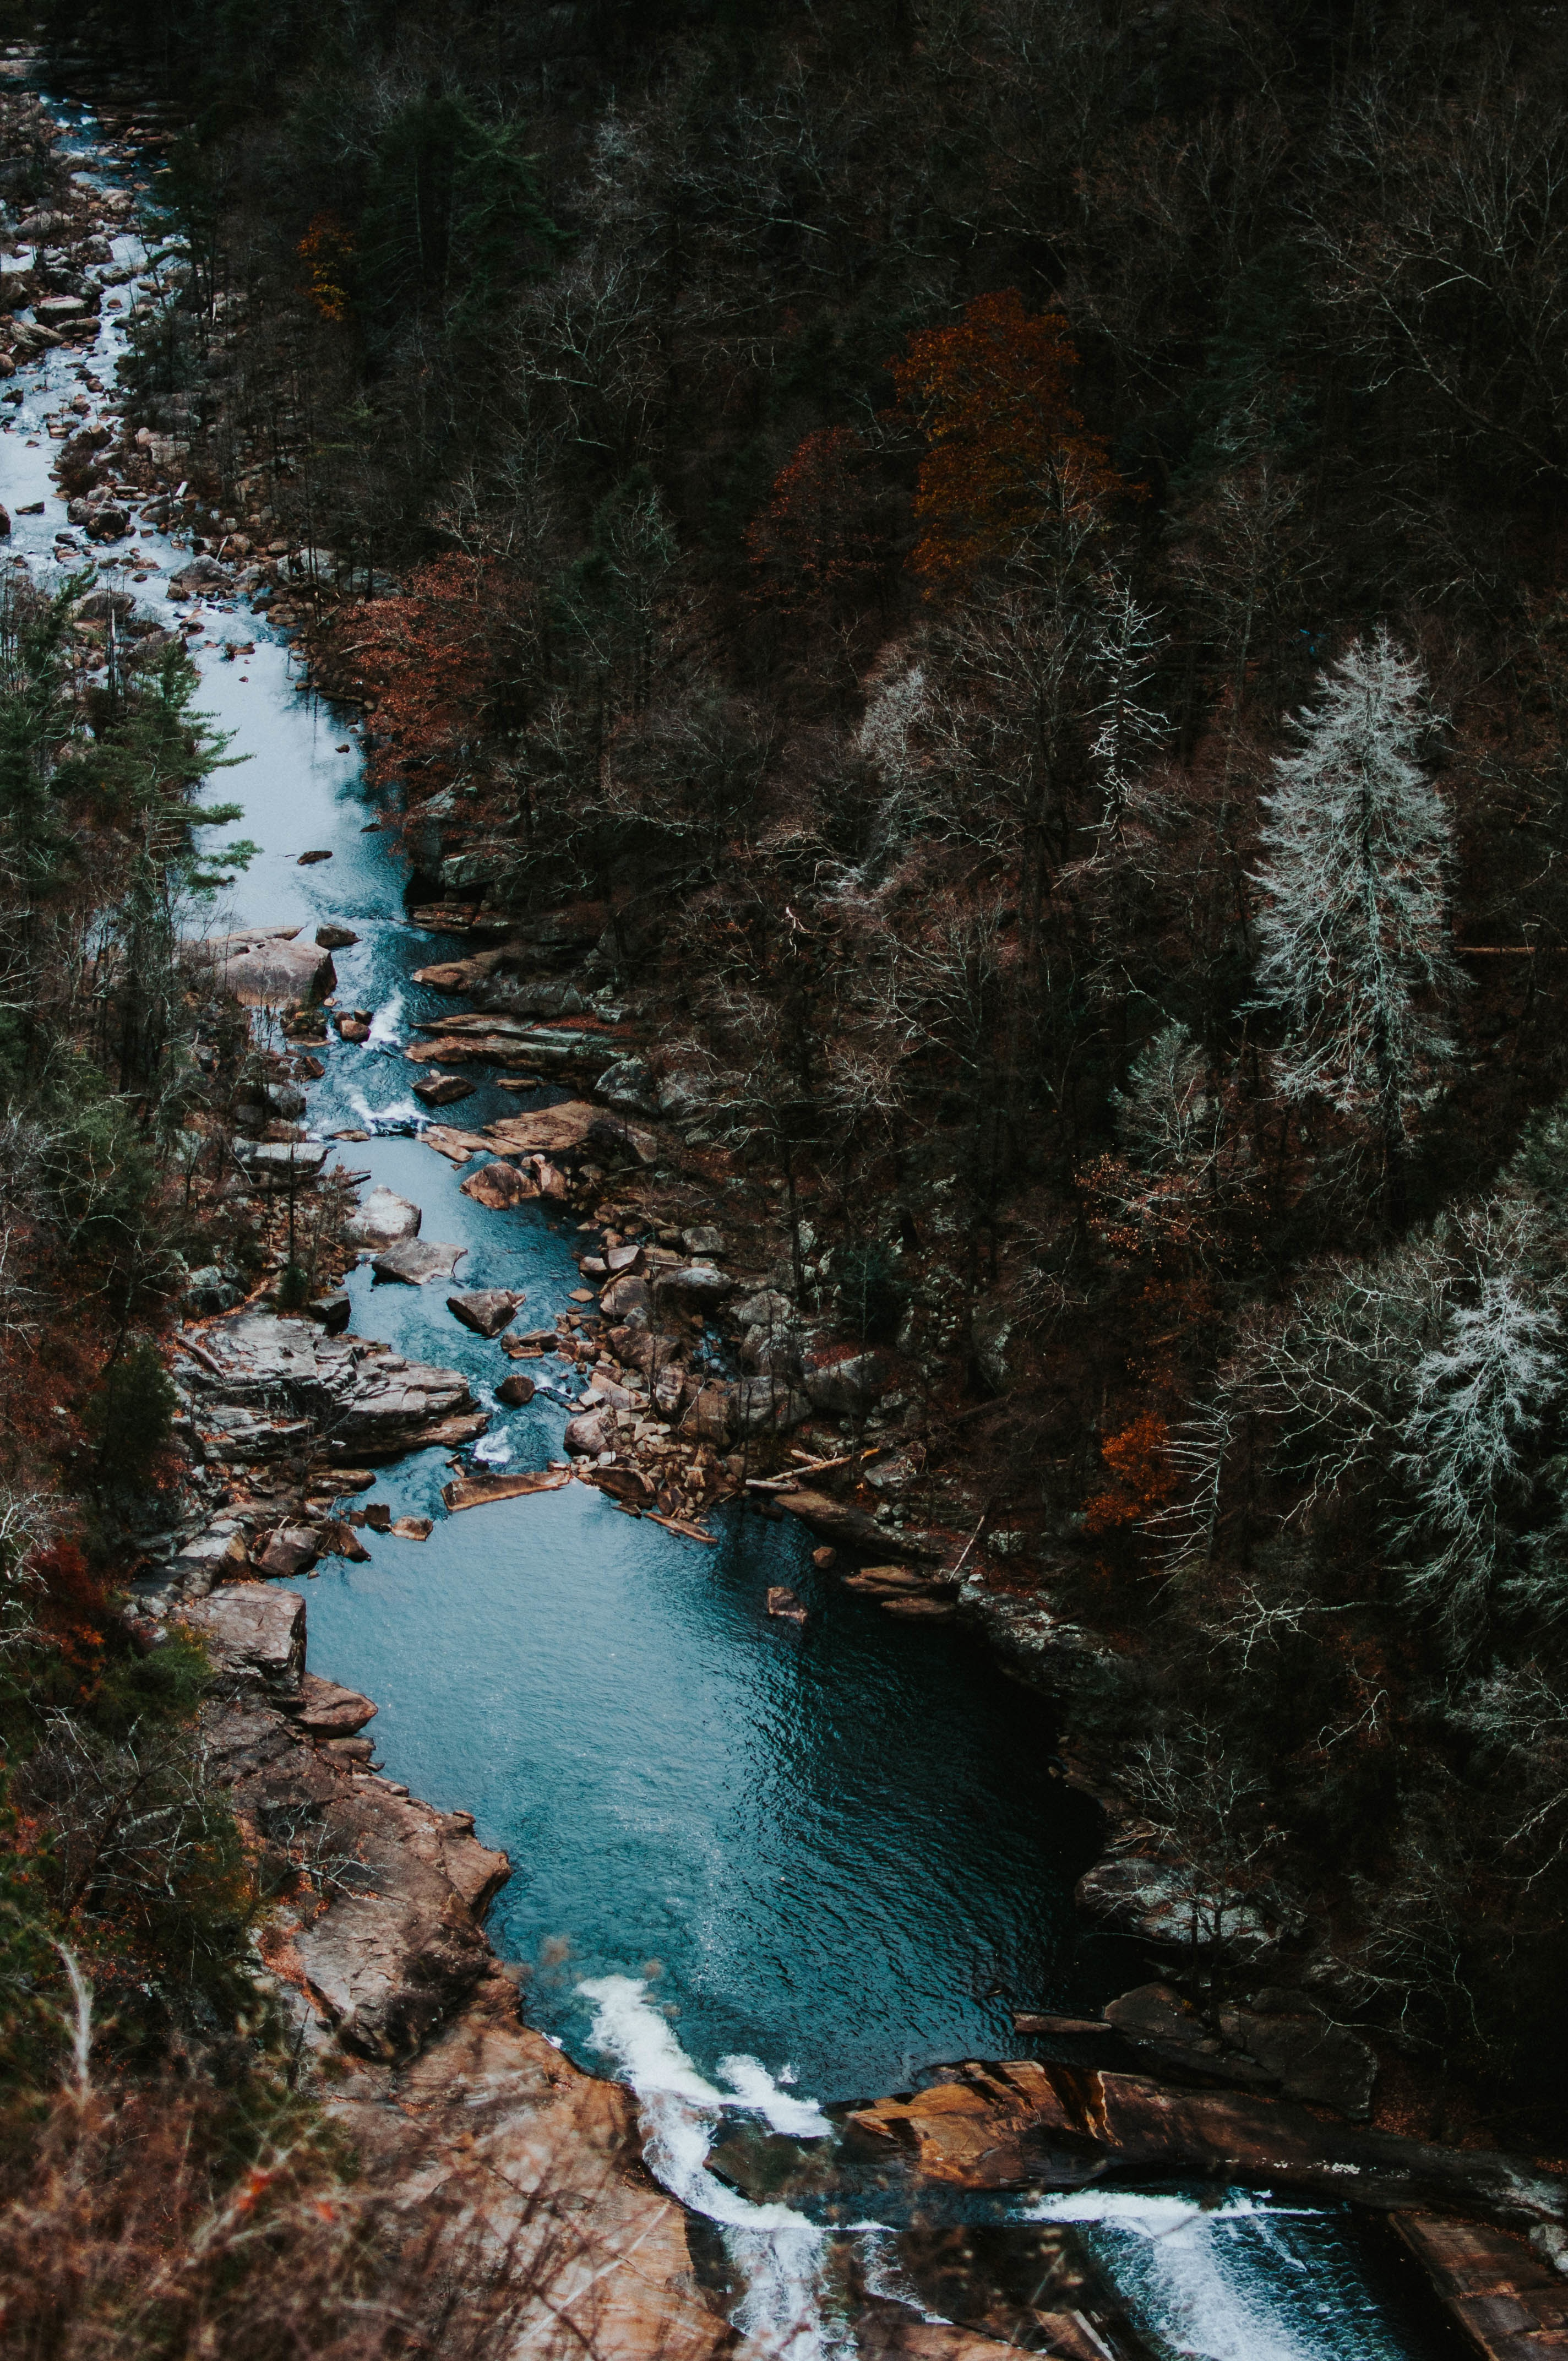
\includegraphics[width=\textwidth]{cover.jpg}
		
		    {\footnotesize Photo By: joanna-kosinska-44214 on unsplash.com } 
			\vspace{1cm}
			
			\textbf{Francisco Navarro Morales - GRG121 }
			
			Segundo curso del Grado de Ingeniería Informática\\
			Universidad de Granada\\
			curso 2016-2017\\
			
		\end{center}
	\end{titlepage}


%\maketitle % Print the title section

%% Resumen (Descomentar para usarlo)
\renewcommand{\abstractname}{Resumen} % Uncomment to change the name of the abstract to something else
%\begin{abstract}
% Resumen aquí
%\end{abstract}

%% Palabras clave
%\hspace*{3,6mm}\textit{Keywords:} lorem , ipsum , dolor , sit amet , lectus % Keywords
%\vspace{30pt} % Some vertical space between the abstract and first section



%%% Inicio del documento

\pagebreak

\section{Como agente reactivo.}
Aunque he reutilizado gran parte del código de la práctica anterior, he modificado muchos aspectos del lado reactivo del agente para obtener mejores resultados. Por ejemplo, he eliminado el comportamiento reactivo que tenía mi agente para abrir puertas siempre que tenía una llave y una puerta a uno de los lados, lo he sustituido por la capacidad de abrir puertas como parte de planes que requieran entrar a ellas, y luego ejecuta la salida como un plan que lleva a un objetivo imaginario que se crea cuando se pasa la puerta en la posición inmediatamente anterior a la puerta(desde donde se entra). He añadido que el agente suelte todos los objetos que tiene poco antes de morir y he modificado la forma en que se actualiza el vector que contiene información sobre qué objetos tiene el agente en cada momento: la idea es poner el elemento correspondiente al objeto que porta a false siempre que realice la acción actTHROW o actPUTDOWN y, en el turno siguiente, comprobar si el objeto activo es nulo y, de no ser así, poner a true el booleano puesto que significaría que no ha sido posible lanzar el objeto.
Un aspecto bastante interesante que he modificado del lado reactivo de mi agente es que he añadido una nueva capa a la parte que decide si girar o seguir adelante para sustituir al método de ir acumulando en una matriz "memoria" el último turno en que se pisó cada casilla y moverse con preferencia por las casillas que se pisaron menos recientemente (o el método de ir sumando uno a la casilla que se va pisando e ir a las que han sido pisadas menos veces). Mi idea ha sido que, dado que el objetivo del agente es \textbf{rellenar todo el mapa}, y no \textbf{pisar todo el mapa}, el criterio que debía seguir, preferentemente, era qué movimiento me desvelaba más casillas por descubrir. Por tanto he programado otra matriz similar a la matriz "memoria" que ya utilizaba en la que sumo uno a cada casilla que ha sido vista en algún momento por el agente y además, tengo una función que determina la suma de los valores de las casillas que serán vistas por el agente si decide avanzar, girar a la izquierda o girar a la derecha. Así, en cada momento comprueba qué movimiento será el que produce un valor menor (y por tanto, el que tiene casillas que han sido vistas menos veces). Esto es especialmente útil para evitar que el agente haga ciclos innecesarios rodeando casillas que \textbf{no ha pisado} pero \textbf{sí ha visto.} No he hecho un estudio exhaustivo de si este método mejora o empeora los resultados porque en la mayoría de los casos el porcentaje de mapa visto fluctuaba en función de si daba la casualidad de que encontraba un objeto determinado antes o después (ya que objetos como las botas o el bikini permiten recorrer el mapa mucho más deprisa) pero aún así los resultados son muy buenos y la impresión que da el agente al ejecutarse es mucho mejor (en mi opinión) que como estaba antes.
Otro detalle es que debido al tamaño de la mochila, que permanece como en la práctica anterior, y que con el añadido de los regalos es insuficiente para llevar todos los objetos a la vez, para no complicarme he decidido que el agente no coja nunca el hueso.

\section{¿Cuando planeo?}
En primer lugar, y principalmente para las etapas del comienzo o después de una muerte, mi agente recoge un conjunto de posiciones con objetos que quiere y no tiene en cuanto los ve y, en cuanto puede, hace un plan para ir a por ellos (Lo he hecho con una búsqueda en anchura porque la implementé antes de implementar el algoritmo de A estrella y me pareció interesante usarla en cortas distancias por ser algo más rápida y sencilla y porque quería darle algún uso). Además de esto, la planificación de ir a por regalos se hace si no se tienen regalos y, para ello, ordeno todos los regalos de los sensores en función de la distancia Manhatan al estado actual e intento ir a por los 3 primeros. Hace lo mismo con los reyes, si tiene regalo, ordena un conjunto de posiciones dónde sabe que hay reyes (si los ha visto) e intenta ir a por los más cercanos. En ambos casos, si no puede encontrar un camino, para evitar que siga buscando en le próximo turno, he programado que pase 30 turnos usando la parte reactiva sin planear.
\section{Algoritmos de búsqueda}
En primer lugar hice una implementación de la búsqueda en anchura, que mejoré para convertirla en el algoritmo A estrella pero que mantuve para distancias cercanas porque consideré que sería más eficiente. En ambos casos he utilizado listas con las acciones que llevan a un estado concreto y, para mejorar la eficiencia en tiempo y facilitar la programación, he utilizado como estructura de datos una cola con prioridad como frontera y un unordered map para almacenar los costes menores para llegar a un nodo y el subplan menor necesario para llegar a dicho nodo. Como estado utilizo tanto la posición como la orientación, de forma que los hijos de un nodo sean el resultado de avanzar o girar a algún lado. He puesto \textbf{un límite de 600 iteraciones de búsqueda} para evitar que haga búsquedas demasiado largas, aunque dado que también hay un límite de distancia antes de iniciar la búsqueda, dudo que se complete demasiado.
La heurística de la búsqueda es la distancia manhatam entre los nodos intermedios y objetivo. Además, algo interesante que he añadido es, cuando se va a introducir en la frontera un nodo que procede de la acción de avanzar, compruebo que no ocurra que el nodo actual y el nodo al que avanza sean uno agua y el otro bosque porque entonces no sería posible avanzar aunque tuviera tanto bikini como zapatillas. En tal caso, el nodo no se añade a la frontera. Además, para evitar que escoja caminos que necesiten equipar y desequipar las botas y el bikini varias veces, he añadido un poco más de coste a los nodos que requieren equipar un objeto (es decir, los que pasan de un terreno normal a agua o bosque).

\end{document}